%
% $RCSfile: data_garden.tex,v $
%
% Copyright (C) 2002-2008. Christian Heller.
%
% Permission is granted to copy, distribute and/or modify this document
% under the terms of the GNU Free Documentation License, Version 1.1 or
% any later version published by the Free Software Foundation; with no
% Invariant Sections, with no Front-Cover Texts and with no Back-Cover
% Texts. A copy of the license is included in the section entitled
% "GNU Free Documentation License".
%
% http://www.cybop.net
% - Cybernetics Oriented Programming -
%
% http://www.resmedicinae.org
% - Information in Medicine -
%
% Version: $Revision: 1.1 $ $Date: 2008-08-19 20:41:06 $ $Author: christian $
% Authors: Christian Heller <christian.heller@tuxtax.de>
%

\subsection{Data Garden}
\label{data_garden_heading}
\index{Data Garden}
\index{Chaos Computer Club}
\index{CCC}
\index{Knowledge Tree}
\index{Data Bush}

Now, if a separation of high-level knowledge from low-level system control
software is considered to be useful, the next question must be:
\textit{How, that is in which form, best to store knowledge in a system?}

One possible structure called \emph{Data Garden} \cite{holland} was proposed by
Wau Holland, founder member and formerly chairman by seniority of the
\emph{Chaos Computer Club} (CCC) \cite{ccc} -- Europe's largest hacker group.
(Note to the reader: A \emph{Hacker} is just a computer freak; a \emph{Cracker}
is a criminal.) Although being a non-academic organisation, his ideas on
knowledge modelling are very interesting to this work. He dreamt of whole
\emph{Forests}, \emph{Parks} or -- as the name says -- \emph{Gardens} of
\emph{Knowledge Trees} and \emph{Data Bushes} (figure \ref{garden_figure}).

\begin{figure}[ht]
    \begin{center}
        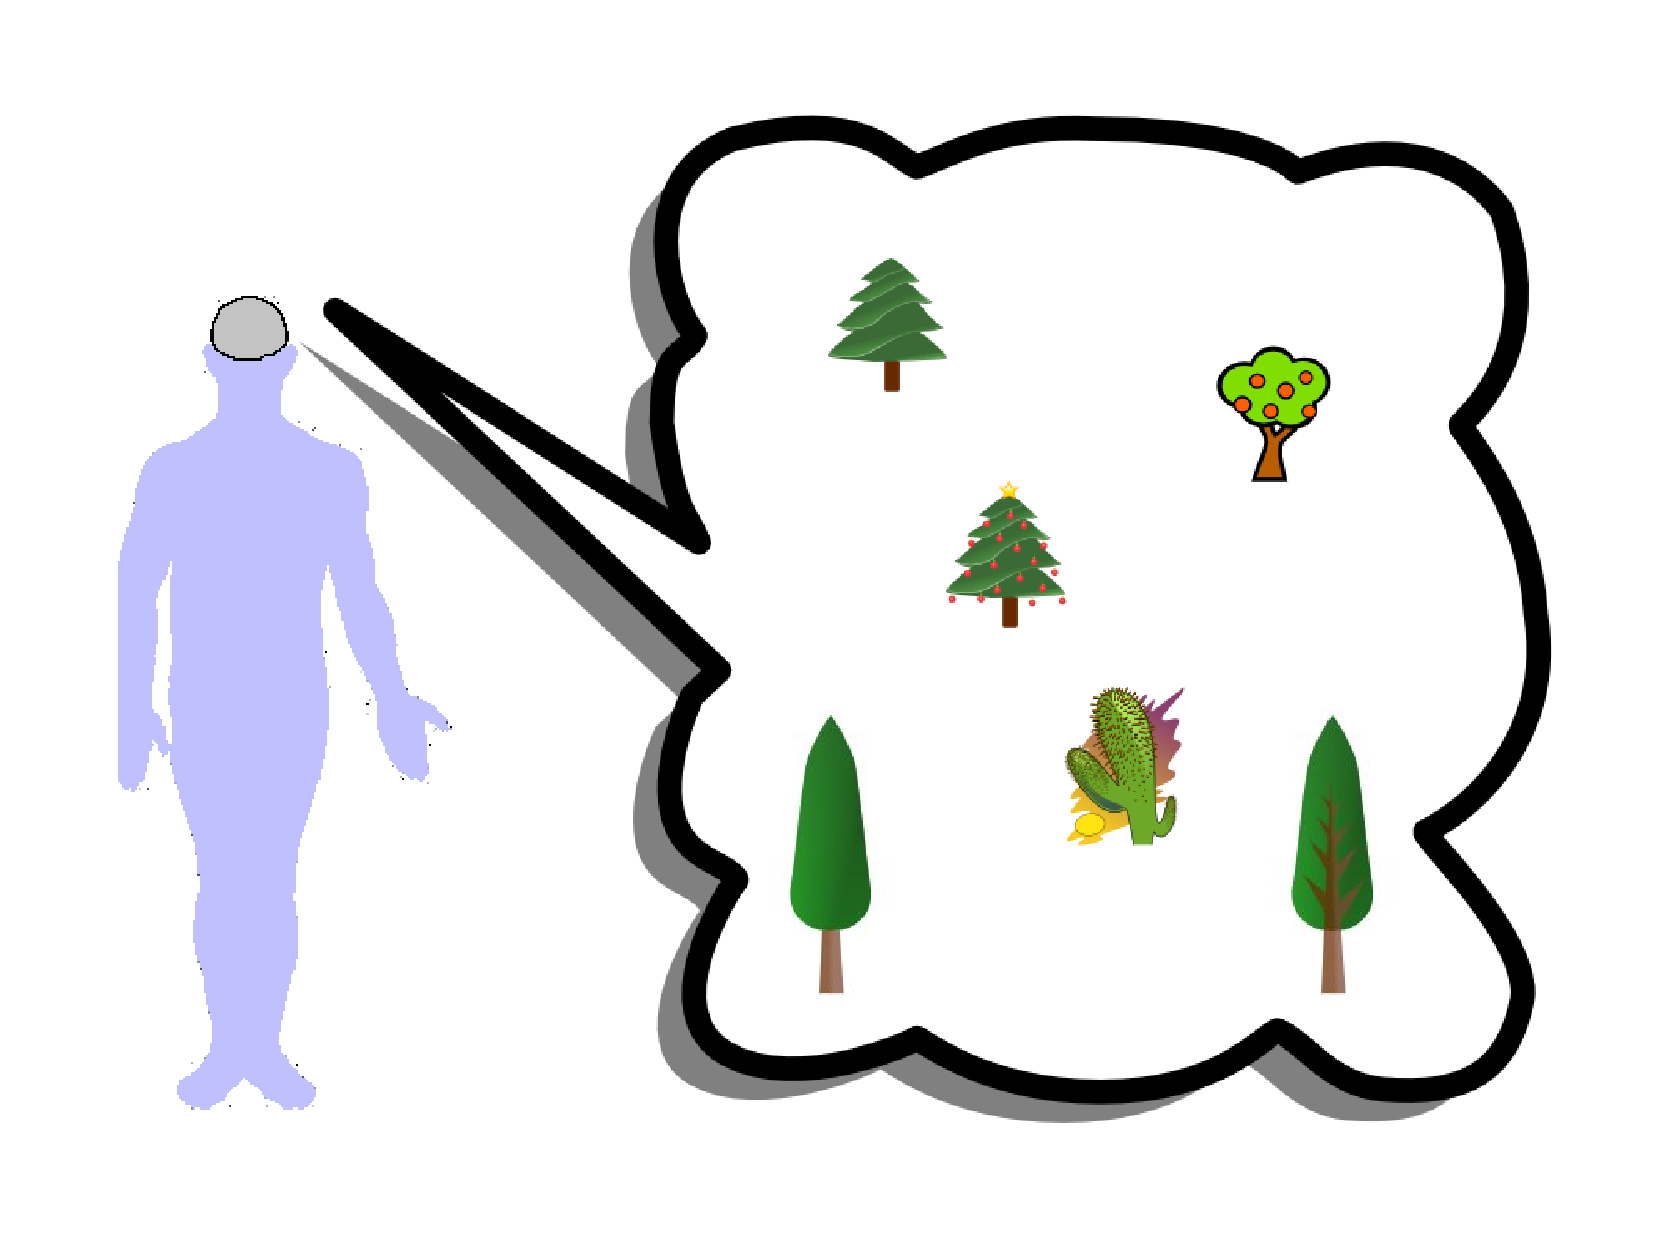
\includegraphics[scale=0.3,angle=-90]{graphic/garden.pdf}
        \caption{Data Garden}
        \label{garden_figure}
    \end{center}
\end{figure}

Many knowledge engineers share a similar view and consider knowledge to be a
network of inter-related concepts. Philippe Ameline writes in
\cite{openehrtechnical}:

\begin{quote}
    All hierarchical trees are inter-connected, and one does better replace
    (purely) \emph{Hierarchical Traits} with \emph{Named Traits} \ldots

    A \emph{Hierarchical Tree} is a set of traits between nodes. These traits
    are not labelled since they all mean \emph{son of}.
    A \emph{Semantic Network} is a set of \emph{labelled} traits, with labels
    of the kind \emph{is a}, \emph{is part of}.

    Thus, building a hierarchy and building a semantic network is the same kind
    of job, but the hierarchy demands two (huge) constraints: there is a
    \emph{Single Root Node}, and nodes have a \emph{Single Kind of Label}.
    These constraints usually can't be satisfied, so a migration from genuine
    hierarchy to semantic network usually occurs.
\end{quote}

The system architecture proposed in this chapter will have \emph{one single}
root node, for all knowledge. Furthermore, chapter \ref{knowledge_schema_heading}
will work out a hierarchical knowledge schema in which \emph{all} parts of a
whole have a unique \emph{Name}.

As an aside: Holland's main interest was the question how information would best
be represented \emph{visually}. Knowledge having the form of plants could be
recognised by their \emph{Shape} or \emph{Colour} which would ease orientation
within a data garden. Old data models that lost in importance could visually
loose their colour or move into the background, becoming smaller in perspective.

Visualisation techniques described in Lombardoni \cite{lombardoni} and Barberena
\cite{barberena} are \emph{Perspective Walls}, the \emph{Benediktine Approach},
\emph{Fractal Rooms}, \emph{Cone Trees} and \emph{Hyperbolic Trees}. In his
work, Lombardoni mapped object-oriented models to three-dimensional graphics.
The techniques are not elaborated further here since they belong to the visual
side of knowledge representation, whilst this work researches concepts for the
structuring, storage and management of knowledge in general. However, the
results of this work might simplify the visualisation of knowledge in future.
Since CYBOP knowledge models are stored in tree-form, it should be rather easy
to represent them graphically.
